\chapter{Método proposto} 

Este capítulo trata da estratégia utilizada para a aquisição das imagens que será utilizada na implementação do algoritmo. Além disso, é definido o escopo e são apresentados detalhes da implementação do método proposto em \cite{Lin:2013}, que serve de base para o mapeamento das distorções avaliadas neste trabalho. Os métodos adotados para a compensação das distorções e montagem do mosaico também  são descritos a seguir.

\section{Plataforma de aquisição}
O experimento será realizado basicamente com três elementos: um objeto cilíndrico de referência (garrafa); uma câmera digital para obtenção das imagens em torno do eixo do objeto cilíndrico; e, por fim, uma plataforma que auxilia no movimento rotacional da garrafa.

O objeto de interesse trata-se de uma garrafa, de vinho, com rótulo frontal e traseiro. Ainda que a produção de vinhos seja substancialmente menor que a produção de cerveja, uma garrafa típica de cerveja tem um formato mais próximo de um cilindro que a garrafa considerada, o que leva a menores distorções e, portanto, a um desempenho melhor dos algoritmos.     

O dispositivo de aquisição utilizado é a câmera traseira de um \textit{smartphone} ASUS, modelo Zenfone 3, com resolução de $4656 \times 2620$ píxeis. A câmera é posicionada para aquisições em formato retrato (\textit{portrait}) a uma distância adequada ao enquadramento integral da garrafa no campo de visão, adicionadas pequenas margens de segurança. 

A garrafa e o sistema de aquisição são colocados em frente a um fundo verde, de forma a gerar uma imagem de alto contraste e de facilitar a segmentação, que não está propriamente no escopo deste trabalho. A câmera (única) é mantida fixa, enquanto a garrafa é rotacionada em passos de $90^\circ$. Com isso, são simuladas aquisições de imagens de uma garrafa fixa a partir de diferentes câmeras.

A rotação da garrafa é implementada com o auxílio de uma plataforma giratória. Essa plataforma possui um formato quadrado com a intenção de facilitar a rotação controlada de $90^\circ$, podendo ser dividida em duas partes, sendo a parte inferior responsável pela fixação e preservação do local em que a plataforma se encontra e a parte superior encarregada de realizar o movimento de rotação da garrafa. Os lados de ambas partes (superior e inferior) sempre permanecem alinhados, garantindo a movimentação correta entre a aquisição das imagens. Na plataforma superior são inseridos marcadores angulares, simulando a posição (angular) das câmeras dispostas em torno do eixo da garrafa. A Figura~\ref{fig:plat_esq} apresenta um esquemático da plataforma utilizada.

\begin{figure}[htb]
    \caption{Diagrama esquemático da plataforma utilizada para a aquisição das imagens. }
    \centering
    \vspace{0.3cm}
    \begin{minipage}{.5\textwidth}
         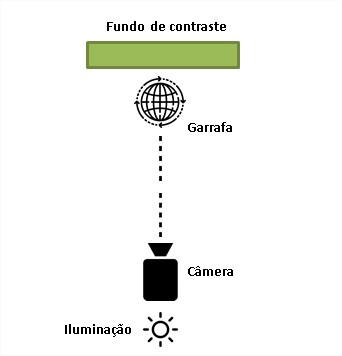
\includegraphics[width=\textwidth]{TCC/Imagens/Esquematico_plataforma.jpg}
         \fonte{O autor (2020).}
	\end{minipage}
    \label{fig:plat_esq}
\end{figure}

\section{Sistema proposto}

Inicialmente, a imagem é submetida a um processo de redimensionamento e seleção da região de interesse. Após esse procedimento, é possível realizar a identificação das distorções de acordo com a quantidade de pontos escolhida pelo usuário. Realizando as compensações geométricas entre os pontos gerados pelo algoritmo, a união das quatro imagens é efetuada, possibilitando uma visão em torno de todo o eixo da garrafa. Um diagrama do sistema proposto é demonstrado na Figura~\ref{fig:diagrama_alg}.

\begin{figure}[htb]
    \caption{Etapas do sistema proposto.}
    \centering
    \vspace{0.3cm}
    \begin{minipage}{\textwidth}
         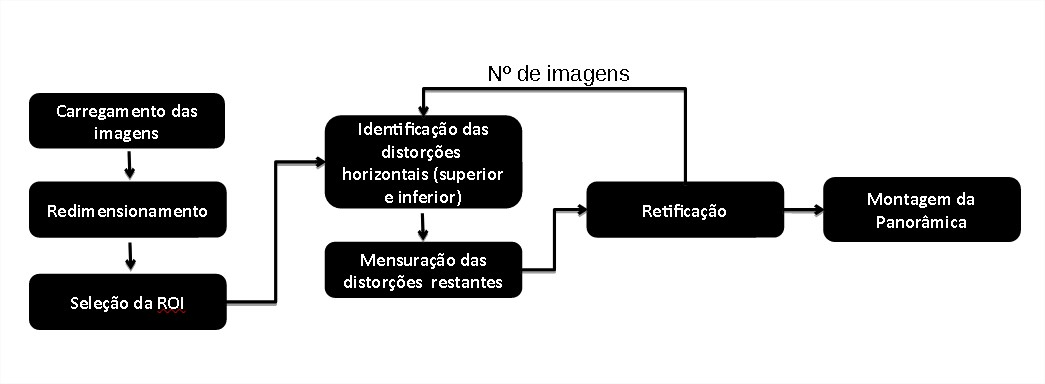
\includegraphics[width=\textwidth]{TCC/Imagens/diagrama_alg.jpg}
         \fonte{O autor (2020).}
	\end{minipage}
    \label{fig:diagrama_alg}
\end{figure}

\section{Pré-processamento da imagem}

As imagens, originalmente com $4656 \times 2620$, são redimensionadas para padrões  HD ($1280 \times 720$). Esse redimensionamento é feito por meio de interpolação bicúbica. São considerados dois tamanhos de imagens para possibilitar uma avaliação da perda de desempenho do método frente à redução da resolução. A redução de dimensão das imagens se dá em função do custo de implementação (o valor de câmera industriais de resolução superior a HD tende a subir significativamente \cite{Webb:2003, Shereena:2015}). Outra razão é a redução no custo computacional, o que, de forma semelhante, impacta nos custos de implementação de um sistema desse tipo.

Seis pontos de interesse, caracterizados pelos limites extremos do maior rótulo (quando observado frontalmente pela câmera) são definidos (por ora, de forma supervisionada). Os pontos que delimitam a região de interesse do algoritmo visam o dimensionamento da elipse causada pela distorção projetiva vertical e são caracterizados pelos seguintes limites (ver Figura~\ref{fig:elipse}):

\begin{enumerate}[label=\arabic*)]
	\item Ponto superior esquerdo;
	\item Ponto de maior ordenada;
	\item Ponto superior direito;
	\item Ponto inferior esquerdo;
	\item Ponto de menor ordenada;
	\item Ponto inferior direito.
\end{enumerate}

Com as coordenadas desses pontos definidas, é possível observar a curva caracterizada geometricamente com o formato de um segmento de elipse, confirmando a representação da distorção afirmada por \cite{Lin:2013}. Na Figura~\ref{fig:elipse} é representado um exemplo da seleção de pontos em uma garrafa em conjunto de uma ilustração da elipse obtida.


\begin{figure}[htb]
    \caption{Pontos que representam as extremidades do rótulo (em amarelo) e a elipse imaginaria (em vermelho).}
    \centering
    \vspace{0.3cm}
    \begin{minipage}{0.4\textwidth}
      \centering
         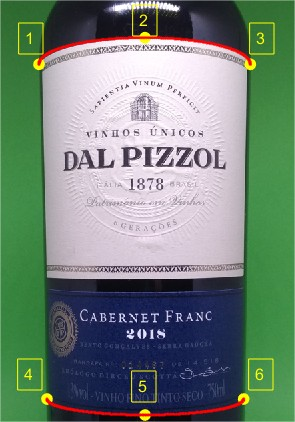
\includegraphics[width=\textwidth]{TCC/Imagens/ellipse.jpg}
         \fonte{O autor (2020).}
	\end{minipage}
    \label{fig:elipse}
\end{figure}

\section{Mapeamento das distorções}

% \cred{<\textit{a pergunta que fica para mim é, precisamos fazer isto?? Não te preocupa com a minha pergunta (depois conversamos sobre isso --- é só para eu me lembrar)}>} 
Para a identificação das distorções projetivas horizontais  e verticais é necessário atribuir a quantidade de pontos horizontais  que  irão representar  o  ``passo'' de ângulo  no  plano  da  imagem.   Uma  quantidade de pontos  maior  proporciona  um  detalhamento  mais  fiel à imagem  planificada,  todavia  isso interfere significativamente no desempenho do algoritmo, demandando um custo computacional mais elevado.
Visto que o mapeamento das distorções é dado pelas equações \eqref{equacao:dist_horz} e \eqref{equacao:dist_vert}, o algoritmo utilizado para a obtenção destas coordenadas é visto no pseudo-código descrito no Algoritmo~\ref{alg:1}.

\begin{algorithm}
    \caption{Mapeamento da Elipse}
    \label{alg:1}
    \begin{algorithmic}[1]
    \Function{map\textunderscore ellipse}{}
    \State $i \gets 1$
    \For{\texttt{$\alpha \gets -\pi/2$ até $\pi/2$ incremente de $\pi/HP$}} \Comment{HP = Pontos horizontais}
        \State $u \gets$ Equação \ref{equacao:dist_horz}
        \If {elipse inferior}
            \State $v \gets$ Equação \ref{equacao:dist_vert} 
        \Else
            \State $v \gets$ $-$ Equação \ref{equacao:dist_vert}
        \EndIf
    \State $Resultado(i) \gets [u, v]$
    \State $i \gets i + 1$
    \EndFor
    \State \Return  $Resultado$
    \EndFunction
    \end{algorithmic}
\end{algorithm}

A variação de $\alpha$ permite obter as coordenadas que representam ambas as distorções.  O que se pode perceber é uma forma geométrica de uma elipse (distorção vertical) com pontos horizontais menos afastados entre si conforme aproximam-se das bordas (limites do rótulo) (distorção horizontal).

Assumindo o diagrama \ref{fig:dist_vert}, nota-se que a caracterização da distorção do eixo vertical vai causando uma perda da excentricidade da elipse conforme se aproxima do centro da figura. Com essa informação é possível concluir que novas elipses devem ser identificadas na área que se delimita aos pontos extremos já conhecidos. 

Para realizar a identificação dos pontos internos (entre as duas elipses estabelecidas supervisionadamente), é possível estabelecer a relação entre as coordenadas das distorções já conhecidas através do pseudo-código transcrito no Algoritmo~\ref{alg:2}, $CES$ e $CEI$ correspondem à coordenada do mesmo ângulo na elipse superior e na elipse inferior, respectivamente.

Basicamente a operação que o algoritmo realiza é a definição de um ''passo'' (que depende da quantidade de pontos verticais), responsável por diminuir a excentricidade da elipse superior. A elipse superior é escrita repetitivamente com a inclinação cada vez menor, até chegar próximo do centro (onde sua inclinação chega muito próxima de zero).

\begin{algorithm}[htb]
    \caption{Mapeamento das demais distorções}
    \label{alg:2}
    \begin{algorithmic}[1]
    \Function{distortion\textunderscore points}{}
     \For{\texttt{$indiceLinha \gets 1$ até $indiceLinha \gets VP$ }} \Comment{VP = Pontos verticais}
         \For{\texttt{$indiceColuna \gets 1$ até $indiceColuna \gets HP$ }} \\
            \State $delta \gets \frac{CES[indiceColuna] - CEI[indiceColuna]}{VP}$ \\
             \State $row[indiceColuna] \gets CES[indiceColuna] - delta * VP$
         \EndFor
        \State $map[indiceLinha] \gets row$
    \EndFor
    \State \Return  $map$
    \EndFunction
    \end{algorithmic}
\end{algorithm}

\section{Compensações das distorções}

Com todos os pontos que representam as distorções existentes no plano da imagem identificados, se vê necessário realizar compensações geométricas a partir deste mapeamento. Para a realização desta tarefa, os valores são armazenados em vetores que representam coordenadas de todos os pontos horizontais a cada índice vertical. A partir deste vetor de armazenamento, sequencialmente, as coordenadas que representam um paralelogramo na imagem, são submetidas a uma transformação geométrica projetiva que irá alterar a forma geométrica (do então paralelogramo), para um bloco com formato retangular com tamanho pré-definido (ver Figura~\ref{fig:quad}).

\begin{figure}[htb]
    \caption{Aplicação da transformada geométrica projetiva no mapeamento das distorções.}
    \centering
    \vspace{0.25cm}
    \begin{minipage}{\textwidth}
      \centering
         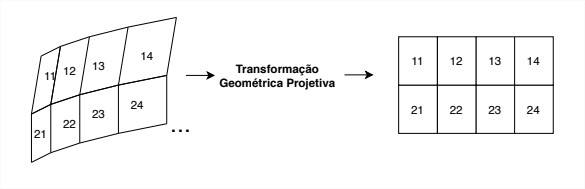
\includegraphics[width=\textwidth]{TCC/Imagens/transform_esq.jpg}
         \fonte{O autor (2020).}
	\end{minipage}
    \label{fig:quad}
\end{figure}


Visando uma representação fiel do rótulo analisado, o dimensionamento da imagem planificada é descrito a seguir. O dimensionado vertical da imagem (planificada) pode ser estabelecido através da distância entre pontos de maior e menor ordenada (definidos pelos pontos atribuídos supervisionadamente). Já o comprimento (total) $C$ da imagem é dimensionado através do tamanho da circunferência que é visualizada na imagem. Utilizando a relação do perímetro da garrafa, é possível definir a largura total da imagem como sendo

\begin{equation}
    C = \frac{2 \pi r}{2} = \pi r
    \label{equacao:largura_imagem}
\end{equation}
em que r, representa o raio da garrafa (em pixels).

Considerando que a imagem total é composta por blocos, cada um deles correspondendo a um ângulo $\alpha$ no plano da imagem original, o dimensionamento horizontal $C$ é dividido igualmente de acordo com a quantidade de pontos horizontais atribuídos. O diagrama da Figura~\ref{fig:esq_bloco} demonstra a lógica que estabelece a compensação geométrica entre os blocos.

\begin{figure}[htb]
    \caption{Esquemático do dimensionamento dos blocos que compõem a imagem.}
    \centering
    \vspace{0.3cm}
    \begin{minipage}{.6\textwidth}
         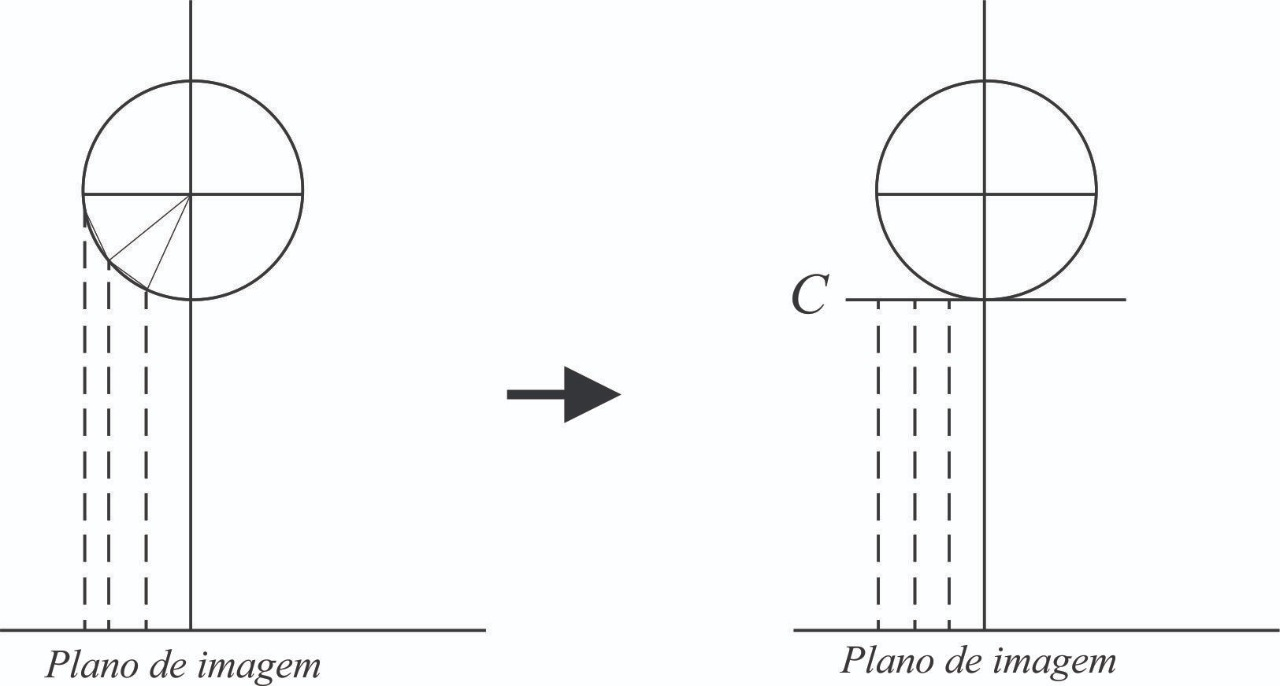
\includegraphics[width=\textwidth]{TCC/Imagens/esq_bloco.jpeg}
         \fonte{O autor (2020).}
	\end{minipage}
    \label{fig:esq_bloco}
\end{figure}

Realizando esse método de compensação com todos os respectivos pontos horizontais e verticais, a imagem planificada é finalmente concluída. Esse procedimento deve ser executado com as demais imagens que representam o deslocamento angular da garrafa, para assim, ser realizada a montagem do mosaico.

\section{Montagem do mosaico}

Diferente do método proposto em \cite{Lin:2013}, que utiliza os algoritmos de registro mencionados no capítulo anterior, neste trabalho optou-se por %utilizar
assumir o movimento da garrafa como conhecido (ou seja, assume-se que a posição das câmeras é conhecida), para realizar a montagem da panorâmica. Os dois principais motivos que justificam a não utilização de algoritmos específicos para o registro de imagens são discutidos a seguir.

Em primeiro lugar, na abordagem de \cite{Lin:2013}, o sistema é empregado para realizar a inspeção em garrafas PET (Polietileno Tereftalato), enquanto neste trabalho avalia-se a inspeção de garrafas que não possuam rótulo que cubra todo o perímetro da garrafa (diferente das garrafas PET, que em sua maioria, apresentam essa característica). Esse detalhe pode vir a impactar diretamente no registro das imagens, visando que as garrafas utilizadas neste trabalho são definidas por grandes áreas de cor homogênea, e a ausência de ``bordas'' e ``cantos'' pode vir a dificultar a detecção de \textit{keypoints} na imagem. Por exemplo, se uma garrafa de vinho não apresentar um rótulo grande o suficiente para compartilhar áreas em comum entre as imagens, o registro pode não conseguir gerar \textit{inliers} o suficiente para calcular uma matriz de homografia responsável por fazer o alinhamento correto das imagens.

O segundo fator aborda o custo computacional exigido pelo algoritmo de registro proposto pelo autor. O método SIFT é constantemente abordado na comunidade científica a fim de propor melhorias de desempenho ao algoritmo, que, apesar de apresentar bons resultados demanda um poder de processamento elevado para detectar os \textit{keypoints} nas imagens \cite{Suzuki:2012}. Somado a isso, na aplicação descrita nesse trabalho deve-se levar em conta o processamento da comparação entre as imagens (minimamente quatro), bem como a transformação e fusão, dificultando a aplicação do método em meio a sistemas de tempo real.

Considerando os problemas descritos, %neste trabalho 
optou-se por assumir que os movimentos relativos entre as imagens são conhecidos. 
A caracterização do movimento conhecido estabelece que o algoritmo já conhece previamente a ordem de arranjo entre as cenas para a montagem do mosaico, bem como a representação angular de cada imagem na panorâmica.

Como já mencionado, o fato deste trabalho estar negligenciando calibrações intrínsecas à câmera e, por isso, cada uma das imagens  planificadas é dimensionada para representar o valor ideal de meio perímetro da garrafa (180$^\circ$), deve ser escolhida a porcentagem de visualização de cada uma das imagens para que cada segmento do mosaico não apresente blocos de imagens repetidos ou faltantes. Assumindo que serão obtidas quatro fotografias em torno do eixo da garrafa, sendo que cada uma dessas representará $90^{\circ}$ de todo o seu perímetro $C$ (idealmente), optou-se pelo descarte de $45^{\circ}$ em cada lado da representação planificada da imagem, assim, a soma da representação angular (na panorâmica) em cada uma das imagens, totalizará o perímetro completo da garrafa.


